\documentclass[11pt]{article}
\usepackage[a4paper,margin=1in]{geometry}
\usepackage{booktabs}
\usepackage{amsmath}
\usepackage[T1]{fontenc}
\usepackage{lmodern}
\usepackage{tikz}
\usetikzlibrary{arrows.meta, positioning, shapes.geometric, fit, backgrounds}
\usepackage[hidelinks]{hyperref}
\setlength{\parskip}{0.4em}
\setlength{\parindent}{0pt}

\title{An Agentic Multi-Method Workflow for Fredholm Integral Equations:\\
\large A Short Report on Results So Far}
\author{Fred-LLM project}
\date{8 July 2026}

\begin{document}
\maketitle

\begin{abstract}
\noindent
We test whether a multi-method agentic workflow helps large language models
solve Fredholm integral equations of the second kind. Five method-specialist
agents propose solutions in parallel, a deterministic SymPy residual check
verifies each one, and a rule-based selector picks the winner without any
further model call. On a 100-equation test set the workflow beats a
single-prompt baseline by 10.6 points on gpt-5.4-mini (21.4\% to 32.0\%), by
1.9 points on the larger gpt-5.4 (36.5\% to 38.4\%), and by essentially nothing
on the top-tier gpt-5.5 (36 correct to 38 of 100). The gain shrinks as the base
model gets stronger. On the stronger models the baseline already solves most of
the winnable problems, so the extra structure has less to recover.
\end{abstract}

\section{Problem}
A Fredholm equation of the second kind has the form
\[
u(x) - \lambda \int_a^b K(x,t)\,u(t)\,dt = f(x).
\]
A person solving one of these usually tries a few standard methods and checks
the candidate solutions against the equation. We built a workflow that imitates
that process with parallel agents, and we measured it against ordinary
single-prompt inference. Both run inside the same evaluation harness, so the two
sets of numbers are directly comparable.

\section{Method}
For one equation the system sends the same problem to five agents, each prompted
to use one technique: separable (degenerate) kernel, Adomian decomposition,
Neumann series, the Fredholm alternative, and a numerical approach. The agents
run at the same time and share nothing. Each returned candidate is then checked
by substituting it back into the equation and measuring the largest residual
$\lvert u(x) - \lambda\int K u\,dt - f(x)\rvert$ at sampled points. A candidate
is \emph{verified} when that residual falls below $10^{-6}$, \emph{failed} when
it parses but misses, and \emph{unverifiable} when it cannot be parsed or the
equation has no checkable form. If nothing verifies, one repair round re-prompts
the failed agents with their own answer and its residual. Selection is
rule-based and calls no model: a verified candidate wins by smallest residual,
otherwise the largest agreeing group wins by majority vote, otherwise the
best-ranked remaining candidate is returned. Because verification and selection
use no model calls, they add no capability that the baseline lacks, which keeps
the comparison fair. The cost is about five to seven model calls per equation
against one for the baseline.

\begin{figure}[h]
\centering
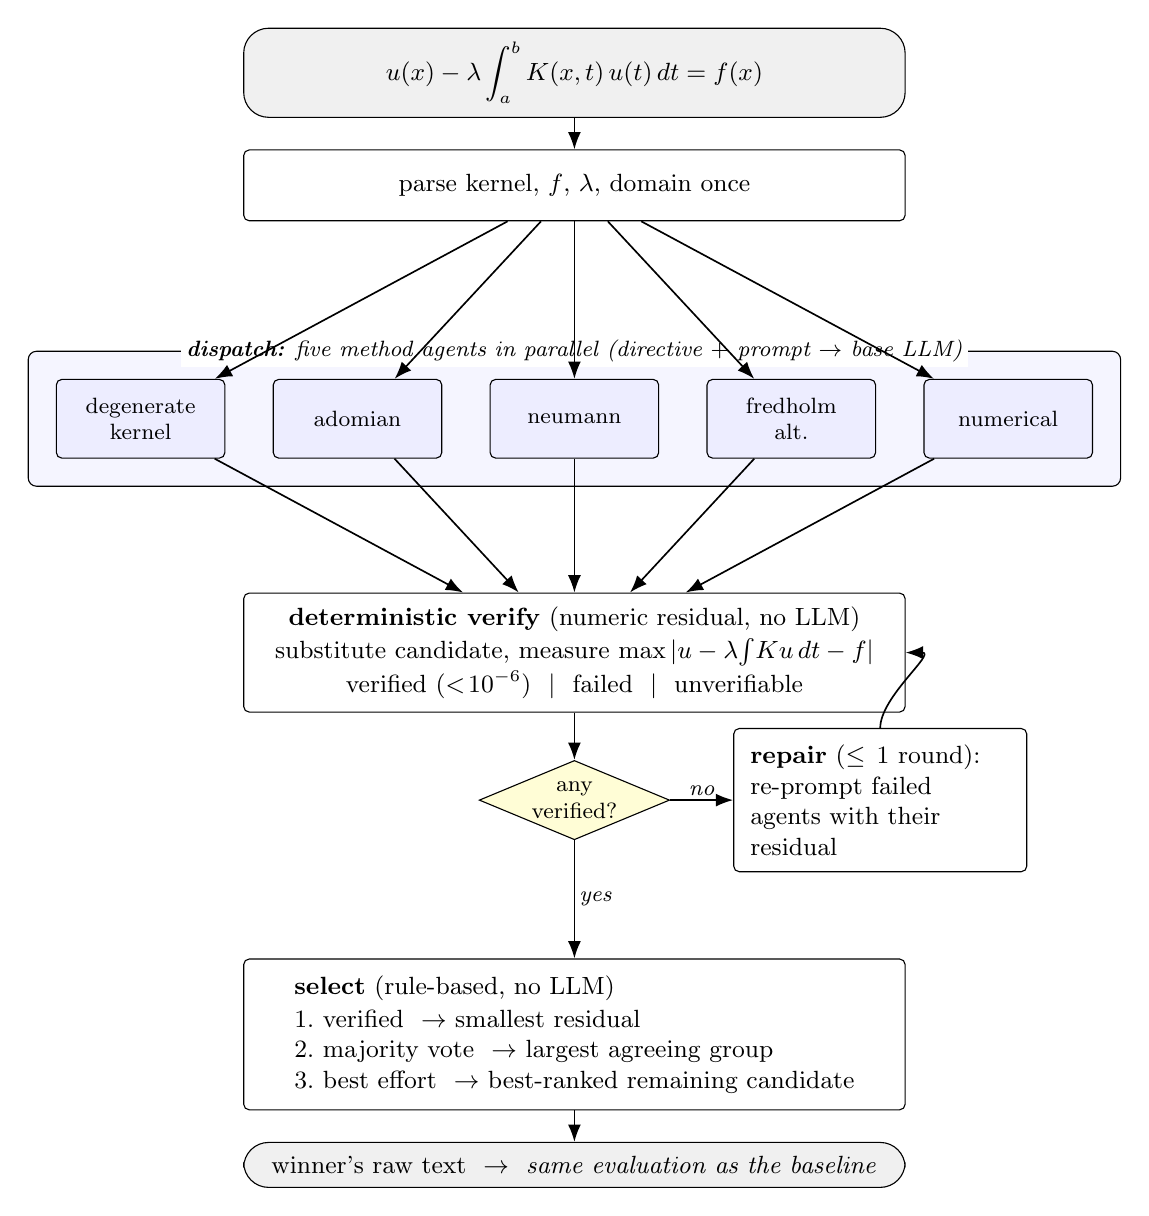
\begin{tikzpicture}[
  font=\small,
  io/.style    ={draw, rounded corners=9pt, fill=black!6, align=center,
                 inner sep=5pt, minimum width=8.4cm},
  proc/.style  ={draw, rounded corners=2pt, align=center, inner sep=5pt,
                 minimum width=8.4cm, minimum height=9mm},
  procL/.style ={draw, rounded corners=2pt, align=left, inner sep=6pt,
                 minimum width=8.4cm},
  agent/.style ={draw, rounded corners=2pt, fill=blue!7, align=center,
                 font=\footnotesize, text width=2.0cm, minimum height=1.0cm,
                 inner sep=2pt},
  dec/.style   ={draw, diamond, aspect=2.4, fill=yellow!16, align=center,
                 inner sep=1pt, font=\footnotesize},
  arr/.style   ={-{Latex[length=2.2mm]}, semithick},
  lbl/.style   ={font=\footnotesize\itshape, inner sep=1.5pt},
]
\node[io] (eq) {$u(x)-\lambda\displaystyle\int_a^b K(x,t)\,u(t)\,dt=f(x)$};
\node[proc, below=4mm of eq] (parse)
  {parse kernel, $f$, $\lambda$, domain once};

\node[agent, below=20mm of parse] (a3) {neumann};
\node[agent, left=6mm of a3]  (a2) {adomian};
\node[agent, left=6mm of a2]  (a1) {degenerate\\ kernel};
\node[agent, right=6mm of a3] (a4) {fredholm\\ alt.};
\node[agent, right=6mm of a4] (a5) {numerical};
\begin{scope}[on background layer]
  \node[draw, rounded corners=3pt, fill=blue!4, fit=(a1)(a5), inner sep=3.5mm]
    (band) {};
\end{scope}
\node[font=\footnotesize\itshape, fill=white, inner sep=2pt] at (band.north)
  {\textbf{dispatch:} five method agents in parallel (directive $+$ prompt $\to$ base LLM)};

\node[proc, below=17mm of a3, minimum height=13mm] (verify)
  {\textbf{deterministic verify} (numeric residual, no LLM)\\[1pt]
   substitute candidate, measure $\max\,\lvert u-\lambda\!\int\! Ku\,dt-f\rvert$\\[1pt]
   verified $(<\!10^{-6})$ \ \textbar\ \ failed \ \textbar\ \ unverifiable};

\node[dec, below=6mm of verify] (dec) {any\\ verified?};

\node[procL, below=15mm of dec] (select)
  {\textbf{select} (rule-based, no LLM)\\[1pt]
   1.\ verified\ \ $\to$\ smallest residual\\
   2.\ majority vote\ \ $\to$\ largest agreeing group\\
   3.\ best effort\ \ $\to$\ best-ranked remaining candidate};

\node[io, below=4mm of select] (out)
  {winner's raw text \ $\to$ \ \emph{same evaluation as the baseline}};

\node[procL, right=8mm of dec, text width=3.3cm, minimum width=0pt] (repair)
  {\textbf{repair} ($\le 1$ round): re-prompt failed agents with their residual};

\draw[arr] (eq) -- (parse);
\foreach \a in {a1,a2,a3,a4,a5} \draw[arr] (parse) -- (\a);
\foreach \a in {a1,a2,a3,a4,a5} \draw[arr] (\a) -- (verify);
\draw[arr] (verify) -- (dec);
\draw[arr] (dec) -- node[lbl, right]{yes} (select);
\draw[arr] (dec) -- node[lbl, above]{no} (repair);
\draw[arr] (repair.north) to[out=90, in=0] (verify.east);
\draw[arr] (select) -- (out);
\end{tikzpicture}
\caption{The agentic multi-method workflow for a single equation. Verification
and selection make no model calls, which keeps the comparison against the
single-prompt baseline fair.}
\label{fig:flow}
\end{figure}

\section{Setup}
Three models were served through an OpenAI-compatible router: cx/gpt-5.4-mini,
cx/gpt-5.4, and cx/gpt-5.5, at temperature 0.1. All are reasoning models; the
gpt-5.4 pair takes roughly 45 seconds per call and gpt-5.5 answers faster. The
test set has 100 equations across seven solution types:
closed-form symbolic, approximate-coefficient, discrete-point, series,
non-unique family, regularized first-kind, and no-solution. Scoring combines
symbolic equivalence, checked with Math-Verify, and numeric residual agreement.
First-kind and no-solution items score on correct type classification instead.
A few model answers are large enough to exceed the evaluator's per-equation time
budget and drop from the denominator, so we report both the correct count out of
100 and the accuracy over the items actually evaluated.

\section{Results}

\begin{table}[h]
\centering
\caption{test\_100 (v2) accuracy, baseline vs.\ agentic, by model.}
\small
\begin{tabular}{lcccccc}
\toprule
 & \multicolumn{2}{c}{gpt-5.4-mini} & \multicolumn{2}{c}{gpt-5.4} & \multicolumn{2}{c}{gpt-5.5} \\
\cmidrule(lr){2-3}\cmidrule(lr){4-5}\cmidrule(lr){6-7}
Metric & base & agentic & base & agentic & base & agentic \\
\midrule
Correct (of 100)        & 21 & \textbf{32} & 35 & \textbf{38} & 36 & \textbf{38} \\
Accuracy (of eval.)     & 21.4\% & 32.0\% & 36.5\% & 38.4\% & 38.3\% & 38.0\% \\
Type accuracy           & 26.4\% & 29.5\% & 38.5\% & 42.0\% & 28.4\% & \textbf{36.7\%} \\
Exact symbolic (of 30)  & 6 & \textbf{13} & 21 & \textbf{24} & 23 & 22 \\
Regularized (of 10)     & 0 & 2 & 1 & 2 & 0 & 1 \\
Family (of 10)          & 10 & 10 & 10 & 10 & 10 & 10 \\
\bottomrule
\end{tabular}
\end{table}

On gpt-5.4-mini the workflow raised accuracy from 21.4\% to 32.0\%. Most of that
came from the closed-form symbolic problems, where verification reliably picks
the correct candidate out of several plausible wrong ones. On gpt-5.4 the same
workflow moved accuracy from 36.5\% to 38.4\%. On gpt-5.5 it moved the correct
count from 36 to 38 of 100, a difference that disappears once the evaluated
denominators are equalized (38.3\% against 38.0\%). Verification fired on 24 of
100 equations for the mini, 33 for gpt-5.4, and 38 for gpt-5.5, so the residual
check settles more equations as the base model improves even while the headline
gain narrows. One thing does keep rising for gpt-5.5: type classification, where
the agentic run adds 8.3 points (28.4\% to 36.7\%). Degenerate-kernel was the
most frequent winning method on all three models. The agentic runs used 713,
735, and 695 model calls respectively.

\begin{table}[h]
\centering
\caption{Model-scaling summary (test\_100 v2).}
\begin{tabular}{lccc}
\toprule
Model & Baseline & Agentic & Lift \\
\midrule
gpt-5.4-mini & 21.4\% (21/98) & 32.0\% (32/100) & \textbf{+10.6 pp / +11 eq} \\
gpt-5.4      & 36.5\% (35/96) & 38.4\% (38/99)  & +1.9 pp / +3 eq \\
gpt-5.5      & 38.3\% (36/94) & 38.0\% (38/100) & $\approx$flat / +2 eq \\
\bottomrule
\end{tabular}
\end{table}

\section{Cost}
The pipeline logs token counts and a cost estimate for every call. The token
counts come straight from each API response and are exact. The dollar figures
are computed from list prices for a gpt-5.4-class model, about \$5 per million
input tokens and \$22.5 per million output, with the mini priced near \$3 per
million blended. These runs went through a custom router, so the dollars are a
proxy for spend rather than the router's actual bill.

\begin{table}[h]
\centering
\caption{Recorded cost of the agentic experiments. Token counts are measured;
dollar figures are list-price estimates for a gpt-5.4-class model.}
\begin{tabular}{lrrr}
\toprule
Run & Requests & Tokens & Cost (USD) \\
\midrule
diverse\_21, three models, baseline        & 63  & 125k  & 1.84 \\
diverse\_21, three models, agentic         & 410 & 978k  & 14.40 \\
test\_100 v2 mini, baseline                & 100 & 181k  & 0.57 \\
test\_100 v2 mini, agentic                 & 713 & 1.61M & 5.12 \\
test\_100 v2 gpt-5.4, baseline             & 100 & 184k  & 3.01 \\
test\_100 v2 gpt-5.4, agentic (recorded)   & 218 & 608k  & 10.62 \\
test\_100 v2 gpt-5.5, baseline             & 100 & 131k  & 3.64 \\
test\_100 v2 gpt-5.5, agentic              & 695 & 1.19M & 34.25 \\
\midrule
Recorded total                             & 2{,}399 & 5.01M & 73.45 \\
\bottomrule
\end{tabular}
\end{table}

Two rows need a note. The gpt-5.4 agentic run resumed from a checkpoint after
an earlier interrupted attempt, so its logged cost covers only the last 28 of
100 equations (218 of about 735 calls). The first 72 equations were paid for in
the interrupted session, which never wrote a summary. Scaling by call count puts
the full gpt-5.4 agentic run near \$36, which raises the true total for all runs
to about \$99 rather than the \$73.45 that was logged. The gpt-5.5 pair, by
contrast, ran end to end and wrote a complete summary, so its \$34.25 is exact
under the proxy pricing. The gpt-5.5 dollars per token also run higher than the
gpt-5.4 figures because the calculator prices that tier above gpt-5.4.

What the accuracy gain costs is the more useful comparison.

\begin{table}[h]
\centering
\caption{Cost of the agentic accuracy gain on test\_100 v2.}
\begin{tabular}{lrrr}
\toprule
Model & Extra cost & Extra correct & Cost per extra correct \\
\midrule
gpt-5.4-mini & +\$4.55        & +11 & \$0.41 \\
gpt-5.4      & +\$33 (est.)   & +3  & \$11 \\
gpt-5.5      & +\$30.61       & +2  & \$15.30 \\
\bottomrule
\end{tabular}
\end{table}

On the mini the agentic run cost about \$4.55 more than its baseline and got 11
more equations right, roughly \$0.41 for each additional correct answer. On
gpt-5.4 the same step cost about \$33 more for 3 more correct answers, roughly
\$11 each. On gpt-5.5 it cost about \$30.61 more for 2 more, roughly \$15.30
each. Cost per unit of accuracy climbs sharply as the base model gets stronger.
That is the accuracy result restated in money: the workflow is a better trade
when the base model is weaker.

\section{Discussion}
The size of the gain tracks the weakness of the base model. gpt-5.4 already
answers 35 of 100 on a single prompt, including 21 of 30 closed-form problems,
so parallel proposal and verification have little left to add. On the mini,
whose baseline gets only 6 of 30 closed-form problems, the same machinery
recovers about twice as many. gpt-5.5 sits at the far end of the same line: its
baseline answers 36 of 100 and the agentic run reaches 38, the same absolute
count the workflow hit on gpt-5.4. Across the three models the lift falls
monotonically, 11 then 3 then 2 more equations, while the agentic output
plateaus and the baseline is what keeps climbing. The verification step works
the same way on all three models and is what drives the closed-form gains. It
simply has more to fix on the weaker model, and by gpt-5.5 there is almost
nothing left. What does not fade is type classification, which the workflow
still improves by 8.3 points on gpt-5.5, and the residual check itself, which
settles more equations on the stronger model even as the headline gain shrinks.

Two limits are worth stating plainly. The evaluated denominators differ a little
between conditions, 96 for the gpt-5.4 baseline and 99 for its agentic run,
because a small number of oversized answers time out of the SymPy scoring; the
correct-count-out-of-100 figures avoid that mismatch. Separately, three solution
types (series, discrete-point, and approximate-coefficient) score near zero for
both conditions across all three models, which caps the available headroom no
matter which method is used.

\section{Conclusion}
The agentic workflow helps, and it helps most where the base model is weakest.
On the stronger models the gain is small enough that the roughly sevenfold
increase in model calls is hard to justify on accuracy alone. Adding the
top-tier gpt-5.5 confirmed the trend the first two models suggested: the lift
fell to about two equations, within the noise of the run, and the cost per extra
correct answer rose to roughly \$15. The workflow remains worthwhile where a
weaker or cheaper base model leaves real headroom, and its verification and
type-classification machinery keeps earning its place even on the strongest
model, but as a way to buy raw accuracy on a capable model it does not pay.

\end{document}
